\chapter{Implementacja}
Implementacja oparta została o minikomputer Raspberry Pi 4B 2GB RAMu. Urządzenie to zostało wybrane arbiralnie - była to platforma która akurat była dostępna "pod ręką". Na minikomputerze zainstalowany został system operacyjny Linux Ubuntu, w wersji $22.04$. System ten był wybrany, jako system wspierany zarówno przez RPi jak i przez środowisko ROS 2. Wersja 22.04 była natomiast najnowszą wersją w czasie rozpoczynania tej części projektu. Bardziej popularny system operacyjny dla tej platformy, czyli Raspbian OS został odrzucony, ponieważ zainstalowanie na nim ROS-a wymaga użycia dockera. Na Ubuntu natomiast wystarczy wykonywać komendy podane wprost w dokumentacji środowiska ROS, co znacznie uprościło podstawową konfigurację środowiska pracy. W celu zdalnego łączenia się z minikomputerem użyty został protokół SSH - po stronie RPi otwarty został serwer SSH, a klient (komputer PC) łączył się z nim przy pomocy aplikacji PuTTY. Dodatkowo do sterowania serwami zastosowany został sterownik Polulu Maestro. Urządzenie to zostało wykorzystane ze względu na dostępność i znajomość obsługi.
\section{Środowisko ROS \cite{ROS_docs}}
Robot Operating System (ROS) to zestaw narzędzi programowych służący do tworzenia aplikacji z myślą o robotach. ROS wprowadza sieć niezależnych, działających równolegle, węzłów (ang. node). Węzły te komunikują się za pomoca tematów (ang. topic), które to stanowią niezmienny interfejs między węzłami. 
Węzły mogą na tematy dane publikować lub je odbierać i implementacja węzła znajdującego się po drugiej stronie nie ma absolutnie znaczenia. Co więcej, nawet nie ma znaczenia czy ten węzeł tam jest. Węzły mogą publikować dane na temty, z których żaden inny węzeł tych danych nie odbiera. Sieć taka jest szczególnie przydatna w przyapdku robotów o pewnym stopniu modularności, bądź w przypadku dowolnych modyfikacji. Zwykle jeden węzeł odpowiada jednemu fizycznemu elementowi robota. Zmiana tego elementu, nawet na element wymagający zupełnie innego oprogramowania, nie jest wtedy problemem. Wystarczy usunąć z sieci odpowiadający mu węzeł i na to miejsce wstawić inny. Jest to bardzo proste, dopóki interfejs (temat na jaki dany węzeł publikuje) pozostaje bez zmian.
\subsection{Schemat implementacji}
\begin{figure}[H]
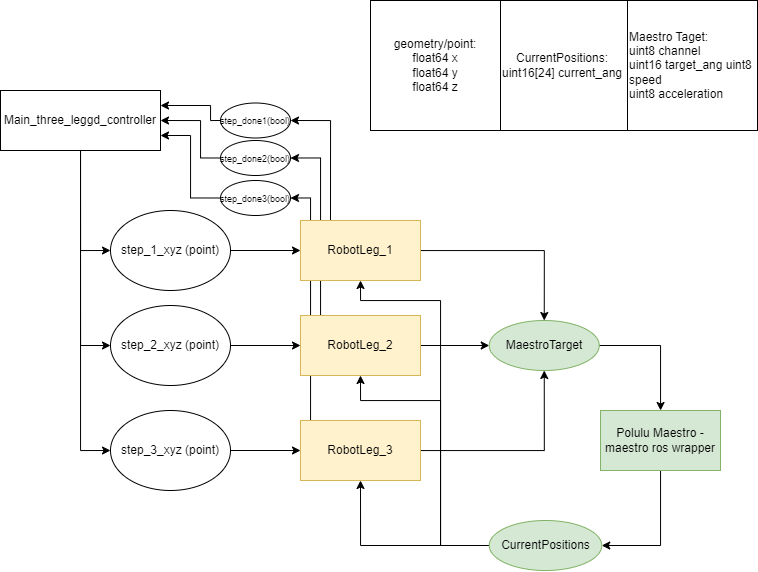
\includegraphics[width=\textwidth]{img/implementation_schematic.png}
\caption{Schemat implementacji w środowisku ROS}
\label{ros_implementation_schematic}
\end{figure}

Rysunek \ref{ros_implementation_schematic} pokazuje schemat komunikacji między poszczególnymi węzłami. Na potrzeby aplikacji zostały stworzone 3 węzły. Jeden odpowiedzialny za obsługę wybranego sterownika do serw, Polulu Maestro, drugi odpowiedzialny za obsługę nogi i trzeci stanowi główny węzeł sterujący. Ma za zadanie generować algorytm chodu i wysyłać polecenia do nóg, aby układały się na docelowe pozycje.
\section{Polulu Maestro 24}
Jest to 24-kanałowy sterownik do serw. Do uruchomienia tego robota wystarczyłby oczywiście Polulu Maestro 12, lecz wersja 24-kanałowa była zakupiona na potrzebny innego projektu i mogła być tutaj wykorzystana bez dodatkowych wydatków. Natomiast steroniki do serw firmy Polulu są wymienne, można w każdej chwili przepiąć serwomechanizmy na sterownik o innej ilości kanałów i dokładnie ten sam program będzie w stanie go także obsłużyć, więc w przyszłości nie będzie problemu z podmianą tego sterownika na mniejszy.\\

Komunikacja ze sterownikiem odbywa się za pomocą protokołu UART Serial. Nie było natomiast potrzeby aby tworzyć wiadomości wysyłane tym protokołem od zera, ponieważ istnieje bilbioteka do komunikacji z tym sterownikiem. Napisana przez Stevena Jackobsa biblioteka Maestro \cite{maestro_pylib} jest szeroko stosowana przy wszelakich projekach z wykorzystaniem tego sterownika i w tym projekcie nie było inaczej. Należało jednak otoczyć tą bibliotekę pewnego rodzaju dekoratorem (ang. wrapper) aby połączyć ją z funkcjonalnościami ROSa. Dlatego napisana została klasa "MaestroRosWrapper" która przez kompozycję zawiera w sobie instancje klasy Maestro z wyżej wymienionej biblioteki Maestro. Stworzona klasa MaestroRosWrapper przede wszystkim implementuje:
\begin{enumerate}
\item Wysyłanie wiadomości co 100ms z odczytem obecnej pozcji wszystkich serw
\item Subskrybowanie wiadomości maestro target, która zawiera informacje o:
\begin{itemize}
\item kanale 
\item pozycji docelowej
\item prędkości
\item przyspieszeniu
\end{itemize}
\end{enumerate}

Na potrzeby tej klasy stworzony został dodatkowy pakiet implementujący dwa customowe interfejsy:
\begin{itemize}
\item MaestroTarget
\item CurrentPositions
\end{itemize}

Są to właśnie te dwa wyżej wspomniane interfejsy, za pomocą których węzeł ten komunikuje się ze światem zewnętrznym.\\

Całość kodu służącego do obsługi tego sterownika została napisana w języku Python 3. Język ten został w tym przypadku wybrany, ponieważ Steven Jackobs zaimplementował swoją bibliotekę w tym właśnie języku. Oczywiście przepisanie jej do innego języka (np. $c++$) nie stanowiłoby dużego problemu, jednakże nie jest to częścią tej pracy. Może to być jednak ciekawe ulepszenie tego projektu, jak węzeł ROS-owy napisany w Pythonie okaże się zbyt pamięciożerny i wolny.
\section{Noga Robotyczna}
Poziom wyżej - nad sterownikiem do serw - znajduje się pojedyncza noga robota. Cały program ją obsługujący był pisany na potrzeby tego projektu zupełnie od zera, co dało zupełną dowolność języka i ogólnej struktury implementacji. \\

Jako język został wybrany c++, z powodu ogólnej preferencji autora programu i aby lepiej zoptymalizować całość robota. Pisanie w języku Python jest znacznie prostsze, ale uruchomienie zbyt wielu węzłów napisanych w tym języku może powodować znaczne problemy z wydajnością.\\

Struktura natomiast, była częściowo wzorowana na poprzednim węźle - sterowniku do serw. Także przyjęto zasadę bardziej "generycznej" klasy wewnętrznej i stricte ROS-owego wrappera. W tym przypadku utworzono klasę Robot Leg przede wszystkim odpowiedzialną za trzymanie informacji o fizycznych parametrach nogi i na ich podstawie przeliczania kinematyk prostej i odwrotnej. Natomiast klasa Robot Leg ROS Wrapper jest odpowiedzialna za komunikację ze "światem zewnętrznym", czyli innymi węzłami ROS-owymi.\\

Najważniejszymi dwoma interfejsami realizowanymi przez ten węzeł jest przyjmowanie nowej pozycji końcówki robota we współżędnych kartezjańskich. Jak tylko takowa się pojawi, przeliczana jest kinematyka odwrotna i publikowana jest pozycja w kątach. Dodatkowo, węzeł ten oczekuje sprzężenia zwrotnego od węzła podrzędnego - operującego sterownikiem. Sprzężenie to jest realizowane przez temat zawierający pozycje wszystkich serw. \\

Węzeł ten powinien także zapewnić sprzężenie zwrotne dla węzła nadrzędnego - tego który publikuje nowe pozycje końcówki nogi. Nie jest to jednak pełne sprzężenie zwrotne, takowe nie byłoby możliwe ze względu na fakt, że kinemtyka odwrotna nie jest idealna - zawiera pewnien błąd (co zostało dokładnie opisane w rozdziale Model Matematyczny/Noga Robotyczna), natomiast kinematyka prosta nie jest tym błędem obciążona. Prawdziwe sprzężenie zwrotne spowodowałoby, że technicznie rzecz ujmując, noga nigdy by nie osiągnęła punktu docelowego. Dlatego zostało ono uproszczone do wymaganego minimum - jak tylko pojawi się informacja o obecnych pozycjach serw (informacja zwrotna od sterownika) i będą one zgodne z pozycjami docelowymi policzonymi za pomocą kinematyki odwrotnej, to węzeł zmienia wartość w temacie step done typu bool na prawdę. (W czasie wykonywania kroku publikowana jest cyklicznie cały czas wartość fałsz.) Taka informacja zwrotna dla węzła nadrzędnego jest jak najbardziej wystarczająca dla poprawnego ruchu robota.\\

\subsection{Poprawki w interfejsach nogi robotycznej}

Aby uczynić węzeł ten bardziej uniwersalnym i ułatwić jego zastosowanie w innych projektach, możnaby dodać dwa dodatkowe tematy na które publikuje ten węzeł - "oszukaną" kinematykę prostą, taką co uwzględnia błąd kinematyki odwrotnej. Dałoby to możliwość zrobienia prawdziwego sprzężenia zwrotnego i liczenia czy krok się faktycznie zakończył wewnątrz węzła nadrzędnego. Byłoby to rozwiązanie bliższe poprawnej "sztuki" implementowania układów sterowania. Dodatkowo warto by było także dodać publikację prawdziwego sprzężenia zwrotnego. Może ono być bardzo przydatne w wielu sytuacjach gdzie potrzebna jest znajomość realnej pozycji końcówki nogi.\\

Innym problemem z interfejsami który wymaga poprawek aby węzeł stał się bardziej uniwersalny są tematy za pomocą których noga komunikuje się ze sterownikiem do serw. Tematy te przenoszą wartości w ćwierć-mikrosekundach, które są jednostką stosowaną przez linię sterowników Polulu Maestro. Powoduje to że konwersja radiany na ćwierć-mikrosekundy jest realizowana już na poziomie nogi robotycznej, a potencjalna wymiana na sterowniki innych producentów może nie być możliwa bez modyfikowania samego kodu nogi. Jest to sprzeczne z ideą ROSa, gdzie wymiana sterownika powinna wiązać się jedynie z wymianą węzła obsługującego ten sterownik. Zamiana tych interfejsów na kąty w stopniach lub radianach i dodanie przeliczania po stronie węzła sterownika poprawiłoby znacznie uniwersalność tej implementacji.\\

Drobnych poprawek wymaga także podział funkcjonalności pomiędzy właściwą klasę RobotLeg a dekorator RobotLegROSWrapper. Jak już wspomniano wcześniej, wrapper ma być odpowiedzialny za komunikację a klasa wewnętrzna za obliczenia. Jednakże na wczesnych etapach implementacji podział ten nie był jeszcze tak jasny i ze względów historycznych, publikacja na temat Maestro Targets jest realizowana przez klasę wewnętrzną. Jest to o tyle problematyczne, że wrapper musi przekazać do kalsy wewnątrz wspólny wskaźnik (Shared Pointer), który wskazuje na publishera na którego temat jest publikowany. Właśnie daltegi i dla spójności implementacji, funckjonalność ta powinna być realizowana przez wrapper nie przez klasę wewnętrzną.\\